\documentclass{beamer}
\newtheorem{remark}{Remark}
\usepackage{hyperref}
\usepackage{array}
\hypersetup{colorlinks,linkcolor=blue}
\begin{document}
\begin{frame}
  \begin{center}
    Deep Learning for Graph Embedding \\
    Section 4.2 of Cai, et. al. \\
  \end{center}

  \vskip 1.5in
  Jeremy Teitelbaum \\
  July 6, 2018
\end{frame}

\begin{frame}{Graph Embedding}
  \begin{problem} Given a (finite, but large) graph $G$ that represents some type of relationship among
    entities, and an integer $n$,  find a map $f:G\to \mathbf{R}^{n}$ that captures interesting features of the graph.
  \end{problem}

  
\end{frame}
\begin{frame}{Deep Learning}
  \begin{definition} \textbf{Deep Learning} is a  buzzword that refers to a class of machine learning algorithms
    that exploit a hierarchical, non-linear structure.
  \end{definition}
\end{frame}

\begin{frame}{Random Walk Methods}
  Random walk embedding methods combine two ideas:
  \begin{enumerate}
  \item Random walks allow one to sample the neighborhood structure of a graph in an efficient way.
  \item Methods developed for natural language processing, applied to samples obtained from random walks, yield a useful graph embedding.
  \end{enumerate}
\end{frame}
\begin{frame}{Random Walks}
  \begin{definition} A (standard) random walk on a graph $G$ is a sequence of vertices $v_0,v_1,\ldots$ of $G$
    constructed so that $v_{i+1}$ is chosen uniformly at random from among the neighbors of $v_{i}$.
  \end{definition}

  \bigskip\noindent
  A random walk is an example of a \textit{Markov Process}, which is a sequence of random variables with the property that the $i^{th}$ random variable depends only on the immediately preceeding one and not the entire history.

  \bigskip\noindent
  There is a huge mathematical literature on such processes.
\end{frame}
\begin{frame}{Example}
  \begin{tabular}{cc}
    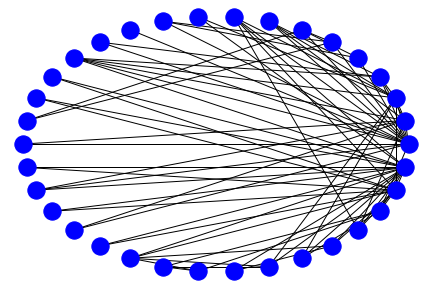
\includegraphics[width=1.8in]{karate.png} &  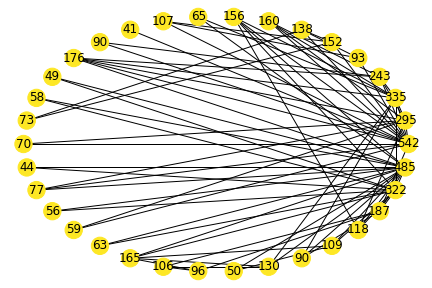
\includegraphics[width=1.8in]{karate_walks.png}\\
    Karate club graph & Graph labelled by number of visits  \\
                                              &by a 5000 step random walk \\
  \end{tabular}
  \begin{remark} In the limit, the number of visits to each node is proportional to the number of neighbors it has.
  \end{remark}
\end{frame}

\begin{frame}{Short random walks capture local structure}
  The following graph shows (American) football games played between Division IA colleges during Fall 2000. Python code for this example is \href{https://networkx.github.io/documentation/stable/auto_examples/graph/plot_football.html}{in the networkx documentation.}
  \begin{center}
    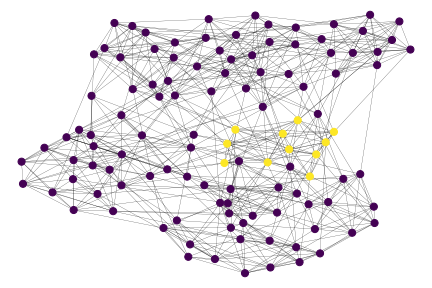
\includegraphics[width=3in]{football.png}
  \end{center}
  \begin{block}{}
    \tiny{ M. Girvan and M. E. J. Newman,
      Community structure in social and biological networks,
      Proc. Natl. Acad. Sci. USA 99, 7821-7826 (2002)}
  \end{block}
\end{frame}
\begin{frame}[fragile=singleslide]{Example of random walks}
  The rows of this table are short random walks from the football graph, showing the team and their conference.  

  \bigskip\noindent
  Most teams play most of their games against their conference, so the short walks stay mostly, but not entirely, within the conference. The 'Big Ten' conference is in yellow.
  
  \tiny{
\begin{verbatim}
Wyoming      [ 7] AirForce     [ 7] Army         [ 4] Tulane       [ 4] Memphis      [ 4] 
Washington   [ 8] UCLA         [ 8] SouthernCali [ 8] OregonState  [ 8] SanDiegoStat [ 7] 
UCLA         [ 8] Stanford     [ 8] NotreDame    [ 5] WestVirginia [ 1] MiamiFlorida [ 1] 
Rice         [11] SanJoseState [11] Tulsa        [11] LouisianaTec [11] LouisianaMon [10] 
Rice         [11] Oklahoma     [ 3] TexasElPaso  [11] NewMexicoSta [10] SouthCarolin [ 9] 
FloridaState [ 0] Maryland     [ 0] NorthCarolin [ 0] Duke         [ 0] Clemson      [ 0] 
VirginiaTech [ 1] WestVirginia [ 1] Temple       [ 1] Navy         [ 5] TexasChristi [ 4] 
Oklahoma     [ 3] Baylor       [ 3] Minnesota    [ 2] Ohio         [ 6] Buffalo      [ 6] 
Stanford     [ 8] SouthernCali [ 8] Oregon       [ 8] SouthernCali [ 8] Stanford     [ 8] 
TexasA&M     [ 3] OklahomaStat [ 3] IowaState    [ 3] Nebraska     [ 3] Iowa         [ 2] 
\end{verbatim}
  }
\end{frame}
\begin{frame}{Local probabilities}

  We try to capture the local structure of the graph by understanding the probability that a node $y$ appears close to a node $x$ in a random walk.

  \bigskip\noindent
  Inspired by work in natural language processing, the authors of DeepWalk suggested considering the probabilities
  $P_{w}(y|x)$   the probability that $y$ occurs somewhere in a random walk of length $w$ that has $x$ in the middle of  it.

\end{frame}
\begin{frame}

  Computing these probabilities in a large network is not feasible. We seek a dimension reduction
  in the form of two maps $$\begin{matrix}n\mapsto u_n \\ n\mapsto v_n\end{matrix}:V\to \mathbf{R}^{k}$$
  with the property that, if $n$ and $m$ are nodes of $V$, then 
  $$
  p(n|m)=\frac{\exp(u_m\cdot v_n)}{\sum_{n} \exp(u_m\cdot v_n)}
  $$
  is a good approximation to the $P_{w}$. Here $u_m\cdot v_n$ is the 'dot product':
  $$
  (u_m^{(1)},u_m^{(2)},\ldots,u_m^{(k)})\cdot (v_n^{(1)},v_n^{(2)},\ldots,u_n^{(k)})=\sum u_{m}^{i}v_{n}^{i}
  $$
  
  The vectors $u_n$ give the graph embedding.

\end{frame}
\begin{frame}{word2vec and SkipGrams}
  The DeepWalk approach is modelled on the word2vec algorithm and the SkipGram concept introduced for natural language processing by Mikolov and his collaborators.

  They associate to every word $w$ in a large vocabulary two vectors $u_w$ and $v_w$ in such a way
  that
  $$
  P(w|w')=\frac{\exp(v_{w'}\cdot u_w)}{\sum_{w} \exp (v_{w'}\cdot u_w)}
  $$
  estimates accurately the probability that if you look in English text and find an occurrence of the word $w'$,
  the chance that $w$ occurs within some fixed distance of $w'$ is $P(w|w')$.
  
  \begin{block}{}
    \tiny{
      Mikolov, et. al. Efficient Estimation of Word Representations in Vector Space. arXiv preprint:1301.3781.
    }
  \end{block}
\end{frame}
\begin{frame}{DeepWalk and  word2vec}
  \begin{tabular}{>{\hangindent=1em}p{2in}>{\hangindent=1em}p{2in}}
    \textbf{word2vec}& \textbf{DeepWalk} \\
    \hline
    Vocabulary & Nodes in a graph \\
    Context of a word & Short random walk centered on a node \\
    Corpus (Text) & Many sampled random walks \\
    Word Vector & Node vector \\
    Probability that a word w occurs near a word v & Probability that a node v is in a short random walk from v' \\
  \end{tabular}
  \end{frame}
  
  \begin{frame}{Maximum Likelihood}
    The vectors $u_m,v_n$ associated to nodes in the graph $G$ are selected by the maximum likelihood principle.

    \bigskip\noindent
    The Likelihood of an observation given a set of probabilities is just the chance of that observation for the given probabilities. In maximum likelihood estimation, one adjusts the probabilities until the likelihood of the observed data is maximal for all possible choices of probabilities.

    \bigskip\noindent
    Suppose that  1000 flips of a coin generate 200 heads and 800 tails.  This is most likely to occur if the probability of a head is $.2$.  That's the maximum likelihood estimate in this case.
  \end{frame}
  \begin{frame}{Stochastic Gradient Descent}
    In the case of word2vec or deepwalk, it is impractical to  directly calculate the maximum likelihood. Instead, one uses an iterative technique to find parameters that are 'good.'  The basic iterative technique is called \textbf{stochastic gradient descent.}

    \bigskip\noindent
    The principle is to look at each sample outcome and compute its likelihood; then to make a small change in the parameters which makes that particular outcome more likely.  Iterating over all the outcomes, the probabilites get moved into the right place.

    \bigskip\noindent
    In the coin flipping example, the idea would be: each time you get an H, move the probability of heads up a bit; each time you get a T, move it down.

    \bigskip\noindent
    If done carefully this will converge to a good estimate of the maximum likelihood.
  \end{frame}
  \begin{frame}{The Football Example}
    We can still run the deepwalk code against the football example, which has 115 teams, and 613 games.  We choose
    an embedding into 20 dimensional space so we end up with 2300 numbers.
    (For reference the adjacency matrix of the graph has about 6500 numbers).

    Applying TSNE to the result we get the following picture, colored by the conference that the teams belong to.
    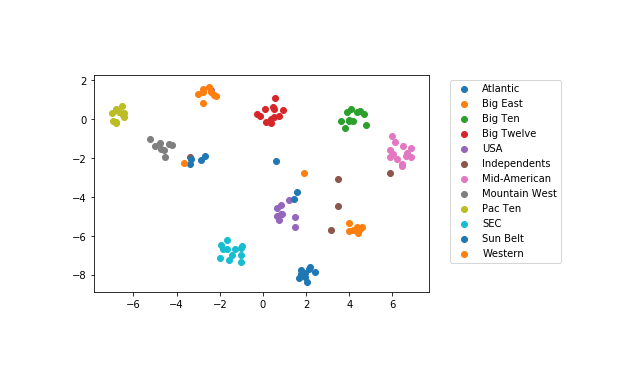
\includegraphics[width=4in]{football_clusters.png}

 \end{frame}
  
    
    
    
\end{document}

%%% Local Variables:
%%% mode: latex
%%% TeX-master: t
%%% End:
